\documentclass{article}

\usepackage[spanish]{babel} % Para que diga 'Figura' en vez de 'Figure'
\usepackage{hyperref}
\usepackage{varioref}
\usepackage{amsmath}
\usepackage[capitalise]{cleveref} % para referenciar figuras, teoremas, etc. de forma automática
\usepackage{geometry} % para cambiar los márgenes
\usepackage{todonotes} % para poner notitas al costado
\usepackage{menukeys} % para poner atajos de teclado
\usepackage{minted} % para poner código fuente con colorcitos
\usepackage{Alegreya} % porque me gusta más esta font
\usepackage{setspace} % para cambiar el espaciado entre líneas
\onehalfspacing % espacio * 1.5
\usepackage{paireddelimiters}


\title{Tips para escribir papers de matemática en \LaTeX}
\author{Eric Brandwein}

\begin{document}
\maketitle

Esta es una guía de las cosas que estuve aprendiendo mientras escribía papers de matemática en \LaTeX. Obviamente va a seguir creciendo infinitamente, y no necesariamente va a estar bien organizada.

\LaTeX\ no es lindo, ni bueno, ni muy comunicativo. Muchas veces te va a aparecer un error, y la única forma de solucionarlo va a ser o googleando, o no haciendo lo que querías hacer. Y podés estar horas al principio para cada pelotudez.\footnote{\href{https://typst.app/}{Typst} trata de solucionar estas cosas, pero no es \LaTeX. Ojalá todos nos pasásemos a Typst.} Solo sabé que esto es normal y no te desesperes.

Hay cosas que directamente no podés hacer con \LaTeX, como por ejemplo agregar emojis. La alternativa es LuaTeX, pero los journals probablemente no te permitan usarlo. Así que por ahora no hay emojis en los papers :(

Esta guía no te va a explicar la sintaxis básica de \LaTeX. Lo mejor para aprender eso son los tutoriales de Overleaf, por ejemplo \url{https://www.overleaf.com/learn/latex/Learn_LaTeX_in_30_minutes}, o directamente ver el código fuente de esta guía en \url{https://github.com/ericbrandwein/tips-latex}.

\newpage
\tableofcontents

\section{Herramientas}
\subsection{Distribución de \LaTeX}
Para compilar \LaTeX\ necesitás una distribución. En Linux, la más común es \href{https://www.tug.org/texlive/}{TeX Live}.

Si estás en ArchLinux o una distribución basada en Arch, podés usar \texttt{pacman} para instalarlo:
\begin{minted}[bgcolor=gray!30]{bash}
 $ sudo pacman -S texlive
\end{minted}
Aunque es mucho más probable que estés usando Ubuntu o una distribución basada en Ubuntu. En ese caso, podés usar \texttt{apt}:
\begin{minted}[bgcolor=gray!30]{bash}
 $ sudo apt install texlive-full
\end{minted}
Si no estás usando ninguna de estas distros, investigalo vos. Y si estás usando Mac o Windows, suerte, no sé nada yo.

\subsection{Editor de texto}
Yo recomiendo usar \href{https://code.visualstudio.com/}{VSCode} con la extensión \href{https://marketplace.visualstudio.com/items?itemName=James-Yu.latex-workshop}{\LaTeX\ Workshop}. Tiene muchas cosas copadas:
\begin{itemize}
    \item Compila automáticamente el documento cada vez que guardás.
    \item Podés ver el PDF generado al lado del código, y podés saltar entre el PDF y el código con SyncTeX. Para saltar del código al PDF, es \keys{\ctrlwin + \Altwin + J}, y al revés es \keys{\ctrlwin + clic izquierdo} (no sé cómo es en Mac, esto es en Linux).
    \item Tiene syntax highlight, así sabés si estás en math mode o no.
    \item Te ayuda un poco con los errores; en general podés ir a Problems y te muestra dónde está el problema. Ver \cref{fig:errores-en-latex-workshop}.
    \item etc. etc. etc.
    \begin{figure}[ht]
        \centering
        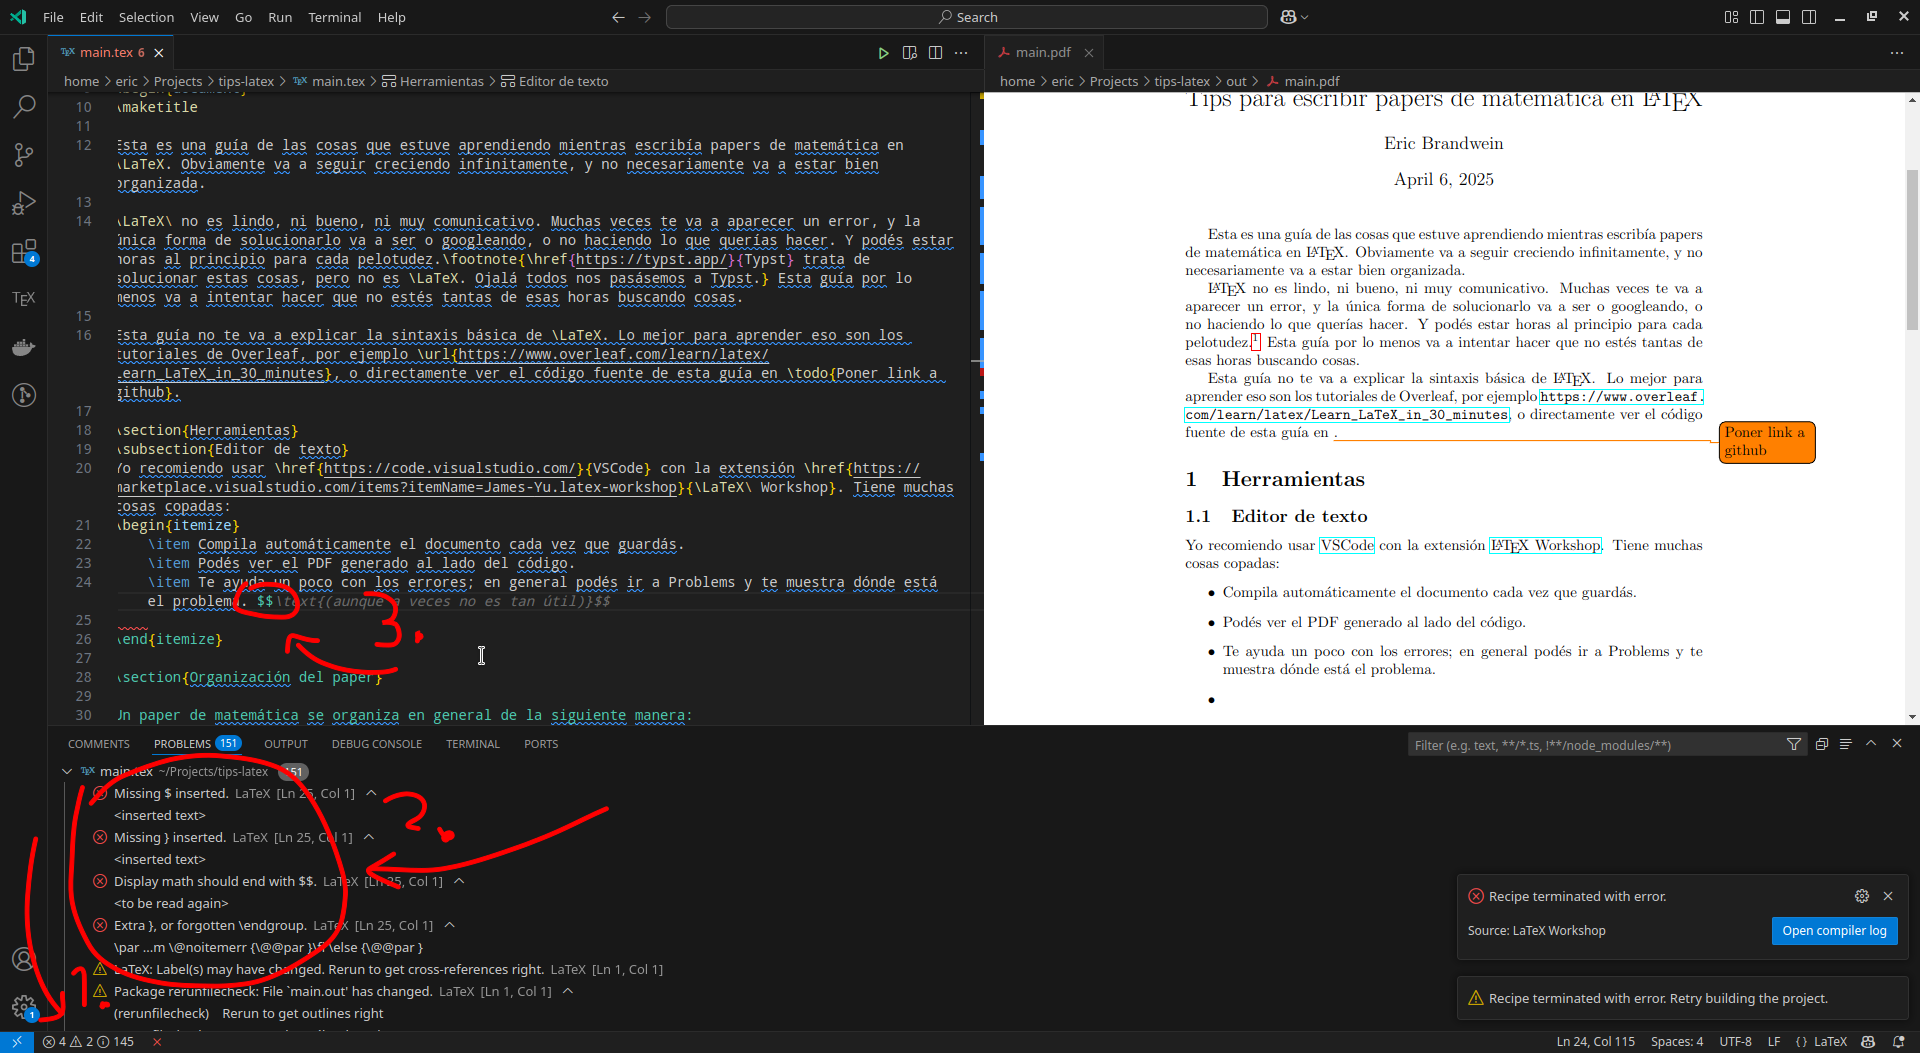
\includegraphics[width=\textwidth]{img/errores-en-latex-workshop.png}
        \caption{Errores en \LaTeX\ Workshop. 1. Dónde cliquear para ver los problemas 2. Los mensajes de error 3. El problema en cuestión: empecé un bloque de matemática con dos \$ y no lo cerré.}
        \label{fig:errores-en-latex-workshop}
    \end{figure}
\end{itemize}

También agregarle la extensión \href{https://marketplace.visualstudio.com/items?itemName=valentjn.vscode-ltex}{LTeX} que te corrige la gramática. Por default te corrige inglés; podés cambiarlo con la configuración \texttt{ltex.language} a \texttt{es-AR}.

Al VSCode le podés también agregar \href{https://github.com/features/copilot}{GitHub Copilot} si te logueás a tu cuenta de \href{https://github.com/}{GitHub}. La verdad que ayuda más en código que escribiendo un paper, pero tiene un chat al que podés preguntarle cosas de \LaTeX\ y a veces te responde bien.

También podés usar \href{https://www.overleaf.com/}{Overleaf}, que es un editor online. Tiene la ventaja de que no tenés que instalar nada, y tiene bastante mejores mensajes de error. Lo malo es que tenés que pagar si querés colaborar con más de una persona creo, y no tenés todo lo que tenés con VSCode. Por ejemplo, si tu proyecto es muy grande, directamente no te deja compilar. Desgraciadamente, la mayoría de los matemáticos usan Overleaf, así que a veces vas a tener que soportarlo. Lo que hago yo es elegir la opción de descargar el código fuente comprimido, descomprimirlo, editarlo en VSCode, y después subir todos los archivos de nuevo al Overleaf.

\subsection{Compilando el PDF}
La extensión de VSCode y Overleaf te compilan solos el PDF. Si querés compilarlo en consola podés usar \texttt{pdflatex}, pero a veces tenés que correrlo muchas veces para que te ponga bien las referencias y otras cosas. Para no tener que hacer eso, lo mejor es usar \texttt{latexmk}:
\begin{minted}[bgcolor=gray!30]{bash}
 $ latexmk -pdf main.tex
\end{minted}

\subsection{Git}
Seguro vas a tener que colaborar con gente si querés avanzar en tu carrera paperística. Y sino, igual vas a escribir cosas, las vas a guardar, te vas a ir a dormir, te vas a despertar, te vas a dar cuenta que no te gustaron, y las vas a querer deshacer, y el \keys{\ctrlwin + Z} no te va a servir. Por eso tenés que usar \href{https://git-scm.com/}{Git}, y subir tus cosas a \href{https://github.com/}{GitHub}. Acá no voy a explicar cómo usar Git, pero si no lo usás y perdés cosas que hiciste y puteás, yo te avisé. El VSCode tiene Git integrado, así que supongo que esa es la forma más fácil de usarlo.

\subsection{Zotero}
\href{https://www.zotero.org/}{Zotero} está bueno para irse guardando los papers interesantes que te encuentres.


\section{Cómo escribir el contenido}
Una muy buena guía para escribir se encuentra en el \href{https://terrytao.wordpress.com/advice-on-writing-papers/}{blog de Terence Tao}. Recomiendo fuertemente leer todos sus posts sobre cómo escribir papers. También recomiendo leer todas las cosas que cita al final, aunque yo no las leí todas.

Para saber lo que se estila a la hora de escribir un paper, lo mejor es leer otros papers. Sin embargo, la mayoría de los papers están escritos para el orto; los papers no están hechos para ser leídos, están hechos para que los resultados sean citados, así que tampoco te copies directamente de lo que leas.
Pero está bueno tener una idea para elegir exactamente qué cosas no copiar.

El objetivo de tu paper es básicamente que te lo publiquen y te lo citen. Una forma de lograr eso es tener resultados importantes, pero si no los tenés, la otra forma es que al que te revise el paper le resulte fácil de leer (para que recomiende su publicación) y que al investigador que se encuentre con tu paper le resulte fácil de leer (para poder aportar en el mismo tema, y por ende citarte). Parece que tenés que escribir un paper que sea fácil de leer. Si tu objetivo no es que te lo publiquen y te lo citen, sino avanzar el conocimiento científico, con más razón querés escribir un paper que sea fácil de leer; si nadie lo puede leer nadie va a ganar mucho conocimiento.

No sé si alguna vez leíste un paper de matemática. Si no lo hiciste lo primero que tenés que hacer es leer uno. Si lo hiciste, seguro te diste cuenta que son \emph{dificilísimos} de leer. Se hace un poco más fácil con el tiempo, pero nunca se vuelve fácil fácil. Siempre vas a leer muchas veces una definición nueva para entenderla, y te vas a olvidar qué significaba después de leer 2 otras.

Pero no tiene que ser tan así. Compará un paper con una charla, o una clase que te hayan dado, o un video, o un artículo de divulgación. ¿Cuáles son las diferencias?
\begin{itemize}
\item\emph{El vocabulario.} Cuando te explican algo se usan palabras simples, y se repiten muchas veces los mismos conceptos para recordarlos. Copiate de esto.
\item\emph{El formalismo.} En general en charlas no te dan las cosas tan formales, matemáticamente hablando. Podés copiarte de esto dando antes de tus resultados una explicación informal de cómo lo vas a demostrar antes de dar la demostración formal.   
\item\emph{La cantidad de imágenes.} En las buenas clases que me dieron, había una imagen por diapositiva más o menos. Es más, había \emph{animaciones}. En PDF no se puede hacer eso, pero sí se pueden poner dibujitos. En mi opinión, las demostraciones deberían tener un dibujo por cada paso, \emph{especialmente} las de grafos. Uno no piensa en grafos con palabras.

Esto atenta contra la máxima cantidad de páginas que te dejan poner en algunas publicaciones. Mi recomendación es hacer los dibujos y sacarlos si no te entran. Siempre se pueden poner en la versión de arXiv.
\item\emph{La subestimación del lector.} Las mejores clases que tuve son en las que el profesor asumía que era un ignorante total. Cuando estés en duda, tirate para abajo en la dificultad. Explicá las cosas obvias, porque son obvias para vos, pero el que va a leer tu paper podría tranquilamente ser uno que está tratando de hacer su tesis de licenciatura y no sabe nada. Es más, seguro que leés de nuevo lo que escribiste en 6 meses y no entendés nada.
\item\emph{La longitud.} Las charlas son cortas, y tu paper va a ser largo. Por eso tenés que repartir tu paper en secciones y subsecciones.
\item\emph{La interactividad.} Lamentablemente el formato PDF no soporta responderte preguntas sobre el paper\footnote{Aunque \href{https://notebooklm.google.com/}{NotebookLM} sí.}, o dejarte hacer ejercicios sobre el tema y decirte si están bien hechos.\footnote{Si se implementasen las ideas de \url{https://willcrichton.net/notes/portable-epubs/} sería un mundo mejor.}
\item\emph{El sonido de la voz de alguien explicándote.} Esto no se puede agregar en un paper lamentablemente, y no sé cuánto ayuda.
\end{itemize}

Entonces, ¿cómo hacer un paper que sea fácil de leer?
\begin{itemize}
\item\emph{No dejar ningún error gramatical.} Usá un grammar checker.
\item\emph{Usar palabras básicas.} Muy lindo lo de querer parecer inteligente, pero mientras tengas un mínimo de formalismo matemático, no hace falta usar palabras rebuscadas. Podés repetir palabras tranquilamente.
\item\emph{Recortar las frases.} Frases largas son más difíciles.
\item\emph{Cagarlo a imágenes.}
\item\emph{Recordar las definiciones que usaste o definiste hace mucho.} La gente se olvida.
\item\emph{Escribir pensando que lo va a leer el vos de hace 6 meses.}
\item\emph{Sin sorpresas.} El que esté leyendo un Lema o una definición tiene que saber por qué lo está leyendo. Tipo, ¿para qué resultado importante voy a necesitar esto que leo? 
\end{itemize}

\subsection{Organización del paper}

Un paper de matemática se organiza en secciones, en general de la siguiente manera:
\begin{enumerate}
\item \textbf{Título, autores, afiliaciones, y funding.}
\item \textbf{Abstract o Resumen.}
\item \textbf{Introduction.}
\item \textbf{Preliminaries.}
\item \textbf{Results.} (No necesariamente con este título, y pueden ser muchas secciones)
\item \textbf{Conclusions.} (Opcional)
\item \textbf{Open problems.} (Opcional aunque no tanto)
\item \textbf{Acknowledgements.}
\end{enumerate}

Paso a explicar qué poner en cada lugar.
\paragraph{Título, autores, afiliaciones, y funding} En general en matemática van los autores en orden alfabético. Las afiliaciones sería la universidad o empresa a la que pertenece cada uno. El funding es la beca o el proyecto de investigación que pagó por que vos labures en el paper.

\paragraph{Abstract} Acá ponés uno o dos párrafos explicando los resultados del paper, o sea, por qué alguien querría leer lo que escribiste. Esto decide si el que lo lea va a meterse a leer el resto del paper, así que es importante que sea claro y conciso. 
\begin{itemize}
\item \textbf{Claro:} Tenés que definir las cosas que necesites para decir el resultado al que llegaste. Nada de hablar de una ``solución consistente apropiada de nivel 2'' sin definir todo eso. Preferentemente, no usar palabras cuya definición que no se pueda leer de otro paper. ¿Por qué es interesante una solución de ese tipo, si no se usa en ningún otro lado?
\item \textbf{Conciso:} Creo que se entiende.
\end{itemize}

En el abstract a veces se pone también un poco de motivación. Tipo, ``el resultado que presentamos avanza en la resolución de un problema abierto en el paper de Fulano'' por ejemplo.

\paragraph{Introduction} Acá ponés un poco de motivación, y decís qué es lo que vas a hacer en el paper. En general, se pone un par de párrafos hablando de los resultados previos en otros papers, y después decís qué es lo que vas a hacer vos. Tratá de llegar lo más rápido posible a tus resultados, y no los demuestres acá, eso va después.

\paragraph{Preliminaries} Acá van las definiciones que vas a usar en todo el paper desde la primera sección. Por ejemplo, decir que los grafos que usamos son no dirigidos y no tienen múltiples aristas, etc. Parafrasear otros preliminaries está bueno, porque casi siempre son muy parecidos. \emph{Ojo: copiarse exacto puede hacer que salten alarmas de plagio cuando lo subas a arXiv o a journals, así que no copies, parafraseá.}

Si hay resultados que se usan en una sola sección, ponerlos justo cuando se empiecen a usar, y no antes. La gente no va a leer los preliminaries, van a ir a tus teoremas y cuando no entiendan algo van a ir a buscar la definición, así que mejor que esté cerquita. 

\paragraph{Results} Esta parte del paper puede tener muchas secciones y subsecciones. Esto es lo más libre del paper. Acá vas a tener tus resultados en forma de:
\begin{itemize}
    \item\emph{Theorems} para los resultados principales de tu paper, los que ponés en el abstract.
    \item\emph{Lemmas} para resultados que necesitás para tus teoremas.
    \item\emph{Corollaries} para resultados que se deducen de los teoremas o lemas.
    \item\emph{Definitions} para definiciones.
    \item\emph{Claims} lo uso para demostraciones adentro de demostraciones.
    \item\emph{Observations} para resultados que son tan fáciles que no necesitan demostración.
    \item\emph{Propositions} que no sé para qué se usan, yo no uso.
\end{itemize}

\paragraph{Conclusions} No es tan usado en matemática, pero si tenés experimentos de algún tipo podés sacar alguna conclusión. Podés también resumir tus resultados en una tabla o algo así.

\paragraph{Open problems} Siempre está bueno poner problemas abiertos que surgen de tu trabajo, porque así ayudás a que tu paper tenga más citas, y eso es todo lo que queremos.

\subsection{Estrategia general de escritura}
La recomendación general es: \emph{¡No te trabes!} Si no te sale escribir algo, escribilo así nomás. Igual vas a tener que releer y reescribir un montón. Por la misma razón, no te podés encariñar con algo que escribiste. Dejalo ir. Casi siempre cuando lo reescribas va a salir mejor.

En particular, me gusta seguir más o menos este orden:
\begin{enumerate}
\item Escribir los statements de los resultados.
\item\label{item:escribir-guia} Escribir una guía en Español de cada demostración.
\item\label{item:escribir-lemas} Identificar qué lemas voy a necesitar para la demo, y escribir los statements.
\item Repetir \cref{item:escribir-guia,item:escribir-lemas} hasta que estén todos los lemas que necesito.
\item Escribir las definiciones en Inglés.
\item Escribir las demostraciones en Inglés.
\item Escribir el texto informal que rodea a los teoremas y ayuda a entenderlos. Incluir ejemplos de aplicación de definiciones y teoremas.
\item Agregar muchas imágenes que ayuden a entender todo.
\item Escribir otras secciones.
\item Escribir la Introducción.
\item Escribir el Abstract.
\end{enumerate}

En el medio, vas a tener que releer todo y reescribir y borrar muchas cosas. Si usás Git está bueno porque no perdés lo que borraste. No tengas miedo de borrar cosas, seguro estaba escrito para el orto y ahora con las ideas claras lo escribís mucho mejor.

El orden no es estricto para nada. Siempre seguí el consejo de no trabarte. Si no tenés ganas de escribir una parte, seguí con otra, y dejá una notita al costado para acordarte de lo que tenías que hacer.

Es necesario que escribas el paper en muchos días diferentes, y que releas lo que escribiste días después. Así vas a saber si se entiende o no. Mientras releas, preguntate: ``¿por qué se cumple esto que dije acá en esta demo?''. Si la explicación que te das a vos mismo no está escrita, escribila. Si implica dibujar algo, dibujalo en el paper. Recordá lo tonto que va a ser tu lector.

Tratá de tener muchos lemas, dividiendo las demostraciones de los teoremas en cachitos.

\section{Usando \LaTeX}
\LaTeX\ funciona con paquetes que se agregan con \verb|\usepackage|. Una distribución completa debería tener todos los paquetes de \href{https://ctan.org/}{CTAN}. Si tenés dudas de cómo usar un paquete, en esa página va a estar la documentación, aunque a veces es más fácil buscar en internet cómo se usa.

El código fuente de esta guía está en \url{https://github.com/ericbrandwein/tips-latex}. Copiate de los paquetes que uso acá para lo que necesites.

También podés copiarte de lo que hacen otros papers. En arXiv te podés descargar el código fuente del paper que quieras. Ver \cref{fig:tex-source-en-arXiv}.

\begin{figure}[ht]
\centering
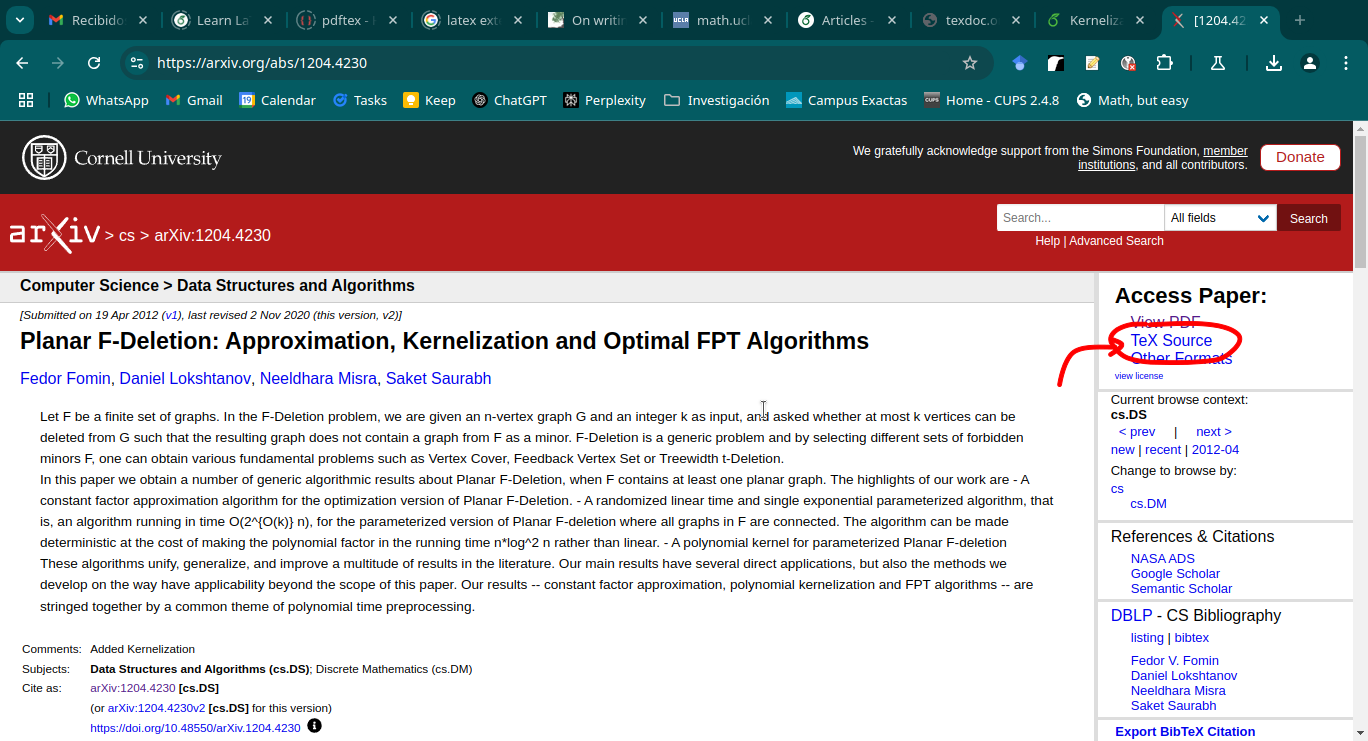
\includegraphics[width=\textwidth]{img/tex-source-en-arXiv.png}
\caption{Código fuente de un paper en arXiv.}
\label{fig:tex-source-en-arXiv}
\end{figure}

\subsection{Citar otros papers}
Hay un montón de paquetes para citar papers en latex. El que más me gusta es \texttt{biblatex}. Leer \url{https://www.overleaf.com/learn/latex/Bibliography_management_in_LaTeX} para una descripción por arriba.

Cosas que descubrí por mi cuenta de \texttt{biblatex}:
\begin{itemize}
\item En vez de \verb|\cite| podés usar \verb|\textcite|, que te pone los nombres de los autores y la cita.
\item Podés citar un teorema en particular de un paper con \verb|\cite[Theorem 1]{paper}|, y te pone ``[Paper, Theorem 1]''. \emph{Siempre poné el número de teorema o de página de donde citás cosas para que sea fácil de encontrar.}
\end{itemize}

Para armar la bibliografía, tenés que crear un archivo \texttt{.bib} y ponerle el nombre que quieras. Yo siempre lo llamo \texttt{references.bib}. Para llenarlo de entradas, podés sacar las citas de Google Scholar, o de \href{https://dblp.org/}{DBLP} si estás haciendo computación. Ojo que hay una diferencia entre citar un paper de un journal y un preprint de arXiv, esto se explica más en \cref{sec:publicar}.

No tengas miedo de ponerles nombres largos a las entradas, nadie lo va a ver, y los editores de texto te autocompletan los nombres en general.


\subsection{Teoremas y definiciones}
Leer \url{https://www.overleaf.com/learn/latex/Theorems_and_proofs}. Los teoremas y los lemas y todo eso deberían todos seguir la misma numeración. Nada de tener una Definition 1 y un Theorem 1 cinco páginas después, eso no ayuda a la búsqueda binaria. Si te descargás el paquete que está en \url{https://github.com/ericbrandwein/latex-packages/tree/main/theoremdefs}, ya te lo resuelve.

La primera vez que escribas el nombre de una cosa que estás definiendo, ponelo en cursiva. Tipo ``Los \emph{números naturales} son los números enteros no negativos''. Después de eso, ya no hace falta ponerlo en cursiva.


\subsection{Referenciar cosas adentro de tu paper}
Cada vez que digas ``Esto se cumple por Lemma 5'', vas a tener que poner un link al Lemma 5. Esto se hace agregando los siguientes paquetes EN ESTE ORDEN EXACTO (sino se rompen cosas):
\begin{minted}[bgcolor=gray!30]{latex}
 \usepackage{hyperref}
 \usepackage{varioref}
 \usepackage{amsthm} % De paso te traés el entorno proof.
 \usepackage[capitalise]{cleveref}
\end{minted}

Después, en donde escribís el lema, ponés

\begin{minted}[bgcolor=gray!30]{latex}
 \begin{lemma}[Teorema de eriquito]
    \label{fact:teorema-de-eriquito}
    $1+1 = 2$.
 \end{lemma}
\end{minted}

y donde lo citás ponés \verb|\cref{fact:teorema-de-eriquito}| y te va a poner ``Lemma 5''. Si querés que te ponga ``Lemma 5 de la página 23'', le ponés \verb|\vref{fact:teorema-de-eriquito}|.

Notar que empiezo el label de los teoremas y lemmas con \verb|fact:|. Algunos diferencian entre teoremas y lemas con \verb|thm:| y \verb|lem:|. Yo prefiero usar \verb|fact:| para toda verdad matemática, porque quizá después pasa a ser un teorema, o un corolario, o lo que sea, y no tengo ganas de cambiar en todos lados el label. Total \verb|\cref| te lo pone bien siempre. Ahora, para definiciones, me gusta usar \verb|def:|, porque ahí sí son cosas diferentes. Para figuras \verb|fig:|, para tablas \verb|table:|, etc.

No importa que los labels sean largos, porque el editor te los autocompleta y el lector no los va a ver.

Ahora, cuando yo leo ``Lemma 5'', no tengo ni puta idea de lo que dice el Lemma 5. Tengo que cliquear el link para acordarme cuál era el lema y después volver a lo que estaba leyendo. En cambio, estaría bueno que en vez de leer ``Lemma 5'', lea ``Teorema de eriquito (Lemma 5)''. Eso es exactamente lo que hace un paquete re pavo que hice que está en \url{https://github.com/ericbrandwein/latex-packages/tree/main/namedtheoremref}. También vas a necesitar descargar el paquete en \url{https://github.com/ericbrandwein/latex-packages/tree/main/theoremdefs}.
Tenés que descargar los \texttt{.sty} y ponerlos en la misma carpeta que tu \texttt{.tex}. Después, lo agregás al preámbulo de tu \texttt{.tex} con:
\begin{minted}[bgcolor=gray!30]{latex}
 \usepackage{namedtheoremref}
\end{minted}

y ponés \verb|\namedtheoremref{fact:teorema-de-eriquito}| y te va a poner ``Teorema de eriquito (Lemma 5)'' con el link al lema y todo.

Con el mismo paquete podés referenciar definiciones por nombre, tipo ``the definition of eriquito (Definition 1)'' para referenciar una definition escrita así:


\begin{minted}[bgcolor=gray!30]{latex}
 \begin{definition}[eriquito]
    \label{def:eriquito}
    \emph{Eriquito} es un doctorando en computación.
 \end{definition}
\end{minted}

\subsection{Imágenes}
Leer \url{https://www.overleaf.com/learn/latex/Inserting_Images}. En general vas a insertar imágenes en un entorno \texttt{figure}.

Para crear las imágenes algo que se usa mucho es \href{https://www.overleaf.com/learn/latex/TikZ_package}{TikZ}. Yo no lo recomiendo. Tardás mucho tiempo en aprenderlo, no hace todo lo que querrías, y hacer una imagen nueva tarda horas, incluso para gente re curtida. Yo primero me pasé a usar \href{https://ipe.otfried.org/}{Ipe}, que es muy fácil de usar, pero tampoco tiene todo lo que quería, así que terminé usando \href{https://inkscape.org/}{Inkscape} con el plugin \href{https://textext.github.io/textext/}{TexText}.

\subsection{Fórmulas}
Todos conocemos el \verb|$...$| y el \verb|\[...\]|. Pero se puede hacer más que eso. Leer \url{https://www.overleaf.com/learn/latex/Aligning_equations_with_amsmath}.

Un detalle es que las fórmulas son parte del texto, así que hay que ponerles un punto final si están al final de la oración. Por ejemplo:
\[1+1=2.\]

Lo mismo pasa con la coma:
\[1+2=3,\]
y la tenés que poner adentro de la fórmula, porque sino te queda abajo y queda feo.

Muchas veces vas a querer escribir algo en una fórmula y no vas a saber cómo. Si hay un símbolo que no sabés cómo escribir, lo mejor es buscarlo en \href{https://detexify.kirelabs.org/}{Detexify}.

No empieces una frase con una fórmula, y separá las fórmulas poniéndoles texto en el medio. En vez de  ``For every graph $G$, $E(G) \subseteq 2^{V(G)}$.'', escribí ``For every graph $G$, we have that $E(G) \subseteq 2^{V(G)}$.'', o algo así.


\subsection{Algoritmos}
Leer \url{https://www.overleaf.com/learn/latex/Algorithms}.

\subsection{Comandos}
A veces vas a usar una letra para un objeto matemático que no te gusta, y la vas a querer cambiar después de haber escrito 10 páginas de tu paper. Por eso tenés que aprender a usar \href{https://www.overleaf.com/learn/latex/Commands}{comandos}. Básicamente lo que hace \LaTeX\ es reemplazar el comando por lo que escribiste.

Por ejemplo, si tenés un grafo $G$ y un subgrafo inducido $H$ de $G$, podés hacer dos comandos:
\begin{minted}[bgcolor=gray!30]{latex}
 \newcommand{\graph}{G}
 \newcommand{\inducedSubgraph}{H}
\end{minted}

y usarlos así:
\begin{minted}[bgcolor=gray!30]{latex}
 For every graph $\graph$, there exists an induced
 subgraph $\inducedSubgraph$ of $\graph$.
\end{minted}

Incluso, mientras estés escribiendo el paper, podés hacer que el comando \verb|\inducedSubgraph| aparezca como \texttt{miGrafoInducido} o algo más declarativo, así es más fácil de leer. Incluso lo podrías dejar así, aunque no muchos van a estar de acuerdo. Si te gusta más $H$ que \texttt{miGrafoInducido}, de vez en cuando está bueno hacer acordar al lector que $H$ es un subgrafo inducido, diciendo por ejemplo ``The induced subgraph $H$ has at most $k$ vertices such that\dots''.

No le tengas miedo a ponerles nombres largos a tus objetos y funciones. Si un número cuenta la cantidad de vértices que cumplen tal propiedad, a mi gusto es mejor $\mathtt{niceVertices}(G)$ que $\alpha(G)$.

\subsection{Múltiples archivos}
Lo mejor es no tener todo el texto en un solo lugar. Especialmente porque muy posiblemente tengas muchas versiones de un mismo paper: una para el journal, otra para un congreso, otra para arXiv, etc. Vas a querer reusar el mismo texto para todas estas versiones, y no tener que estar copiando y pegando. Para eso, podés usar el paquete \texttt{import}. Leer \url{https://www.overleaf.com/learn/latex/Management_in_a_large_project}.

\subsection{Otros paquetes}
\begin{itemize}
    \item\href{https://tug.ctan.org/macros/latex/contrib/todonotes/todonotes.pdf}{\texttt{todonotes}} -- Para poner notas al lado del paper.\todo{Tipo así.}
    \item\href{https://github.com/ericbrandwein/latex-packages/tree/main/paireddelimiters}{\texttt{paireddelimiters}} -- Delimitadores comunes, tipo \verb|$\set{G \mid \abs{V(G)} > 2}$| se ve tipo $\set{G \mid \abs{V(G)} > 2}$. Para que se vea bien cuando tenés cosas grandes adentro, hay que poner un \texttt{*}. Ver diferencias entre estas dos fórmulas:
    \begin{align*}
        &f\parens{\sum_{i = 1}^{20} i^2}\\
        &f\parens*{\sum_{i = 1}^{20} i^2}
    \end{align*}
    \item\href{https://texdoc.org/serve/geometry.pdf/0}{\texttt{geometry}} -- Para cambiar los márgenes y el tamaño de página. No se usa mucho en journals porque ya te lo definen ellos. Leer \url{https://www.overleaf.com/learn/latex/Page_size_and_margins}.
    \item\href{https://ctan.org/pkg/minted?lang=en}{\texttt{minted}} -- Para poner código fuente con colorcitos. Leer \url{https://www.overleaf.com/learn/latex/Code_Highlighting_with_minted}.
    \item Muchos más, no voy a poner todos.
\end{itemize}


\section{Cómo publicar}
\label{sec:publicar}

¡Felicitaciones! Escribiste tu paper y ahora querés que el mundo lo vea. Para eso tenés que mandarlo a una \emph{revista} (\emph{journal}) para que ellos llamen a otros investigadores que lo revisen (haciendo \emph{peer review}) y decidan si recomiendan publicar tu paper en el journal o no. Esto va a tardar unos meses entre que lo enviás, los reviewers te mandan correcciones, las corregís, y se repite esto hasta que o te lo aceptan o te lo rechazan.

Hay algunos journals que tienen más \emph{impacto} que otros, medido por ejemplo en la cantidad de citas que tiene uno de sus papers en promedio. Cuanto mayor es el impacto, más difícil es publicar ahí, y más prestigio (CV) te da publicarlo ahí. Cuanto más CV, mejores chances de que te admitan para becas y para posiciones académicas en el futuro.

Los journals de mayor impacto dependen de cada área. Probablemente tu director de tesis te pueda ayudar a elegir uno.

Como los journals tardan un montón, en computación lo que se hace mucho es publicar en un congreso antes de publicar en un journal. En estos vos mandás una versión reducida de tu paper (un \emph{extended abstract}), y si te lo aceptan, lo presentás en una charla en el congreso. A veces si no te entran las demostraciones de los resultados podés agregarlas a un apéndice con \verb|\appendix|. Tenés que pagar para ir al congreso aunque vos presentes algo, y alguien te tiene que pagar el costo de los pasajes y la estadía si es en otro país.

También lo que hacen todos es publicar una versión preliminar (un \emph{preprint}) a \href{https://arxiv.org/}{arXiv}. Casi cualquiera puede subir cualquier cosa a arXiv, así que lo mejor es citar de un journal si está disponible, que por lo menos se supone que están un poco más revisados.

Cada journal va a tener un template de \LaTeX\ que vas a tener que descargar y llenar. También van a haber instrucciones para los autores de cómo escribir el paper.

Las políticas de publicación de papers en journals, congresos y arXiv pueden ser complicadas. En general, mandar un paper a un journal te prohíbe mandar a otro journal hasta que el primer journal te rechace el paper. Para saber si podés mandar a un journal al mismo tiempo que mandás a un congreso tenés que leer las condiciones de cada uno a ver si son compatibles. Por otro lado, en general no podés subir a arXiv la versión publicada en un journal. Lo que sí podés hacer en general es subir la versión con las últimas correcciones que hiciste antes de que lo publiquen, que obviamente va a ser casi lo mismo.

Si avanzás un poco más en tu carrera quizá te piden que vos revises un paper de alguien más. Tené en cuenta que no te van a pagar ni te van a dar crédito por hacerlo, porque es anónimo. Además, vas a tardar unos días en leerlo y en entenderlo. Lo que ganás es que tenés acceso más rápido a nuevos resultados, aunque como dije, todos primero publican en arXiv, así que esa ventaja es leve. Si tu puesto es de profesor, probablemente te lo pidan como parte de tu trabajo. Si no, no es necesario que lo hagas, pero una buena forma de aprender a escribir papers es corregir a alguien más.

Y sí, los journals te cobran por descargar los papers, y los que revisan no ganan un peso, y los autores tampoco. Por eso en un momento \href{https://www.theguardian.com/science/2017/jun/27/profitable-business-scientific-publishing-bad-for-science}{generaban más ingreso que Google, Apple, y Amazon} (y no sé si lo siguen haciendo). Te ofrecen publicar sin que el que lo lea tenga que pagar, pero para eso tenés que pagar vos. Y no es 10 pesos que tenés que pagar; es \href{https://www.elsevier.com/about/policies-and-standards/pricing#1-publishing-charges}{miles de dólares} por paper. Todo por el \emph{prestigio} de la revista. No sé si se nota el odio que le tengo al sistema científico actual, enganchado al pasado cuando los papers se imprimían, no queriendo soltar el chupete. Pero así es la situación actual.


\end{document}